\documentclass[twoside]{book}

% Packages required by doxygen
\usepackage{fixltx2e}
\usepackage{calc}
\usepackage{doxygen}
\usepackage[export]{adjustbox} % also loads graphicx
\usepackage{graphicx}
\usepackage[utf8]{inputenc}
\usepackage{makeidx}
\usepackage{multicol}
\usepackage{multirow}
\PassOptionsToPackage{warn}{textcomp}
\usepackage{textcomp}
\usepackage[nointegrals]{wasysym}
\usepackage[table]{xcolor}

% Font selection
\usepackage[T1]{fontenc}
\usepackage[scaled=.90]{helvet}
\usepackage{courier}
\usepackage{amssymb}
\usepackage{sectsty}
\renewcommand{\familydefault}{\sfdefault}
\allsectionsfont{%
  \fontseries{bc}\selectfont%
  \color{darkgray}%
}
\renewcommand{\DoxyLabelFont}{%
  \fontseries{bc}\selectfont%
  \color{darkgray}%
}
\newcommand{\+}{\discretionary{\mbox{\scriptsize$\hookleftarrow$}}{}{}}

% Page & text layout
\usepackage{geometry}
\geometry{%
  a4paper,%
  top=2.5cm,%
  bottom=2.5cm,%
  left=2.5cm,%
  right=2.5cm%
}
\tolerance=750
\hfuzz=15pt
\hbadness=750
\setlength{\emergencystretch}{15pt}
\setlength{\parindent}{0cm}
\setlength{\parskip}{3ex plus 2ex minus 2ex}
\makeatletter
\renewcommand{\paragraph}{%
  \@startsection{paragraph}{4}{0ex}{-1.0ex}{1.0ex}{%
    \normalfont\normalsize\bfseries\SS@parafont%
  }%
}
\renewcommand{\subparagraph}{%
  \@startsection{subparagraph}{5}{0ex}{-1.0ex}{1.0ex}{%
    \normalfont\normalsize\bfseries\SS@subparafont%
  }%
}
\makeatother

% Headers & footers
\usepackage{fancyhdr}
\pagestyle{fancyplain}
\fancyhead[LE]{\fancyplain{}{\bfseries\thepage}}
\fancyhead[CE]{\fancyplain{}{}}
\fancyhead[RE]{\fancyplain{}{\bfseries\leftmark}}
\fancyhead[LO]{\fancyplain{}{\bfseries\rightmark}}
\fancyhead[CO]{\fancyplain{}{}}
\fancyhead[RO]{\fancyplain{}{\bfseries\thepage}}
\fancyfoot[LE]{\fancyplain{}{}}
\fancyfoot[CE]{\fancyplain{}{}}
\fancyfoot[RE]{\fancyplain{}{\bfseries\scriptsize Generated by Doxygen }}
\fancyfoot[LO]{\fancyplain{}{\bfseries\scriptsize Generated by Doxygen }}
\fancyfoot[CO]{\fancyplain{}{}}
\fancyfoot[RO]{\fancyplain{}{}}
\renewcommand{\footrulewidth}{0.4pt}
\renewcommand{\chaptermark}[1]{%
  \markboth{#1}{}%
}
\renewcommand{\sectionmark}[1]{%
  \markright{\thesection\ #1}%
}

% Indices & bibliography
\usepackage{natbib}
\usepackage[titles]{tocloft}
\setcounter{tocdepth}{3}
\setcounter{secnumdepth}{5}
\makeindex

% Hyperlinks (required, but should be loaded last)
\usepackage{ifpdf}
\ifpdf
  \usepackage[pdftex,pagebackref=true]{hyperref}
\else
  \usepackage[ps2pdf,pagebackref=true]{hyperref}
\fi
\hypersetup{%
  colorlinks=true,%
  linkcolor=blue,%
  citecolor=blue,%
  unicode%
}

% Custom commands
\newcommand{\clearemptydoublepage}{%
  \newpage{\pagestyle{empty}\cleardoublepage}%
}

\usepackage{caption}
\captionsetup{labelsep=space,justification=centering,font={bf},singlelinecheck=off,skip=4pt,position=top}

%===== C O N T E N T S =====

\begin{document}

% Titlepage & ToC
\hypersetup{pageanchor=false,
             bookmarksnumbered=true,
             pdfencoding=unicode
            }
\pagenumbering{roman}
\begin{titlepage}
\vspace*{7cm}
\begin{center}%
{\Large My Project }\\
\vspace*{1cm}
{\large Generated by Doxygen 1.8.11}\\
\end{center}
\end{titlepage}
\clearemptydoublepage
\tableofcontents
\clearemptydoublepage
\pagenumbering{arabic}
\hypersetup{pageanchor=true}

%--- Begin generated contents ---
\chapter{Black\+Jack}
\label{md_README}
\hypertarget{md_README}{}
This is a simple library of c++ files that allow the user to start and play games of Black Jack with a variable number of players and sets of cards in the playing deck. 
\chapter{Hierarchical Index}
\section{Class Hierarchy}
This inheritance list is sorted roughly, but not completely, alphabetically\+:\begin{DoxyCompactList}
\item \contentsline{section}{Board}{\pageref{class_board}}{}
\item \contentsline{section}{Card}{\pageref{class_card}}{}
\begin{DoxyCompactList}
\item \contentsline{section}{Ace}{\pageref{class_ace}}{}
\end{DoxyCompactList}
\item \contentsline{section}{Deck}{\pageref{class_deck}}{}
\item \contentsline{section}{Hand}{\pageref{class_hand}}{}
\item \contentsline{section}{Player}{\pageref{class_player}}{}
\end{DoxyCompactList}

\chapter{Class Index}
\section{Class List}
Here are the classes, structs, unions and interfaces with brief descriptions\+:\begin{DoxyCompactList}
\item\contentsline{section}{\hyperlink{class_ace}{Ace} }{\pageref{class_ace}}{}
\item\contentsline{section}{\hyperlink{class_board}{Board} }{\pageref{class_board}}{}
\item\contentsline{section}{\hyperlink{class_card}{Card} }{\pageref{class_card}}{}
\item\contentsline{section}{\hyperlink{class_deck}{Deck} }{\pageref{class_deck}}{}
\item\contentsline{section}{\hyperlink{class_hand}{Hand} }{\pageref{class_hand}}{}
\item\contentsline{section}{\hyperlink{class_player}{Player} }{\pageref{class_player}}{}
\end{DoxyCompactList}

\chapter{Class Documentation}
\hypertarget{class_ace}{}\section{Ace Class Reference}
\label{class_ace}\index{Ace@{Ace}}
Inheritance diagram for Ace\+:\begin{figure}[H]
\begin{center}
\leavevmode
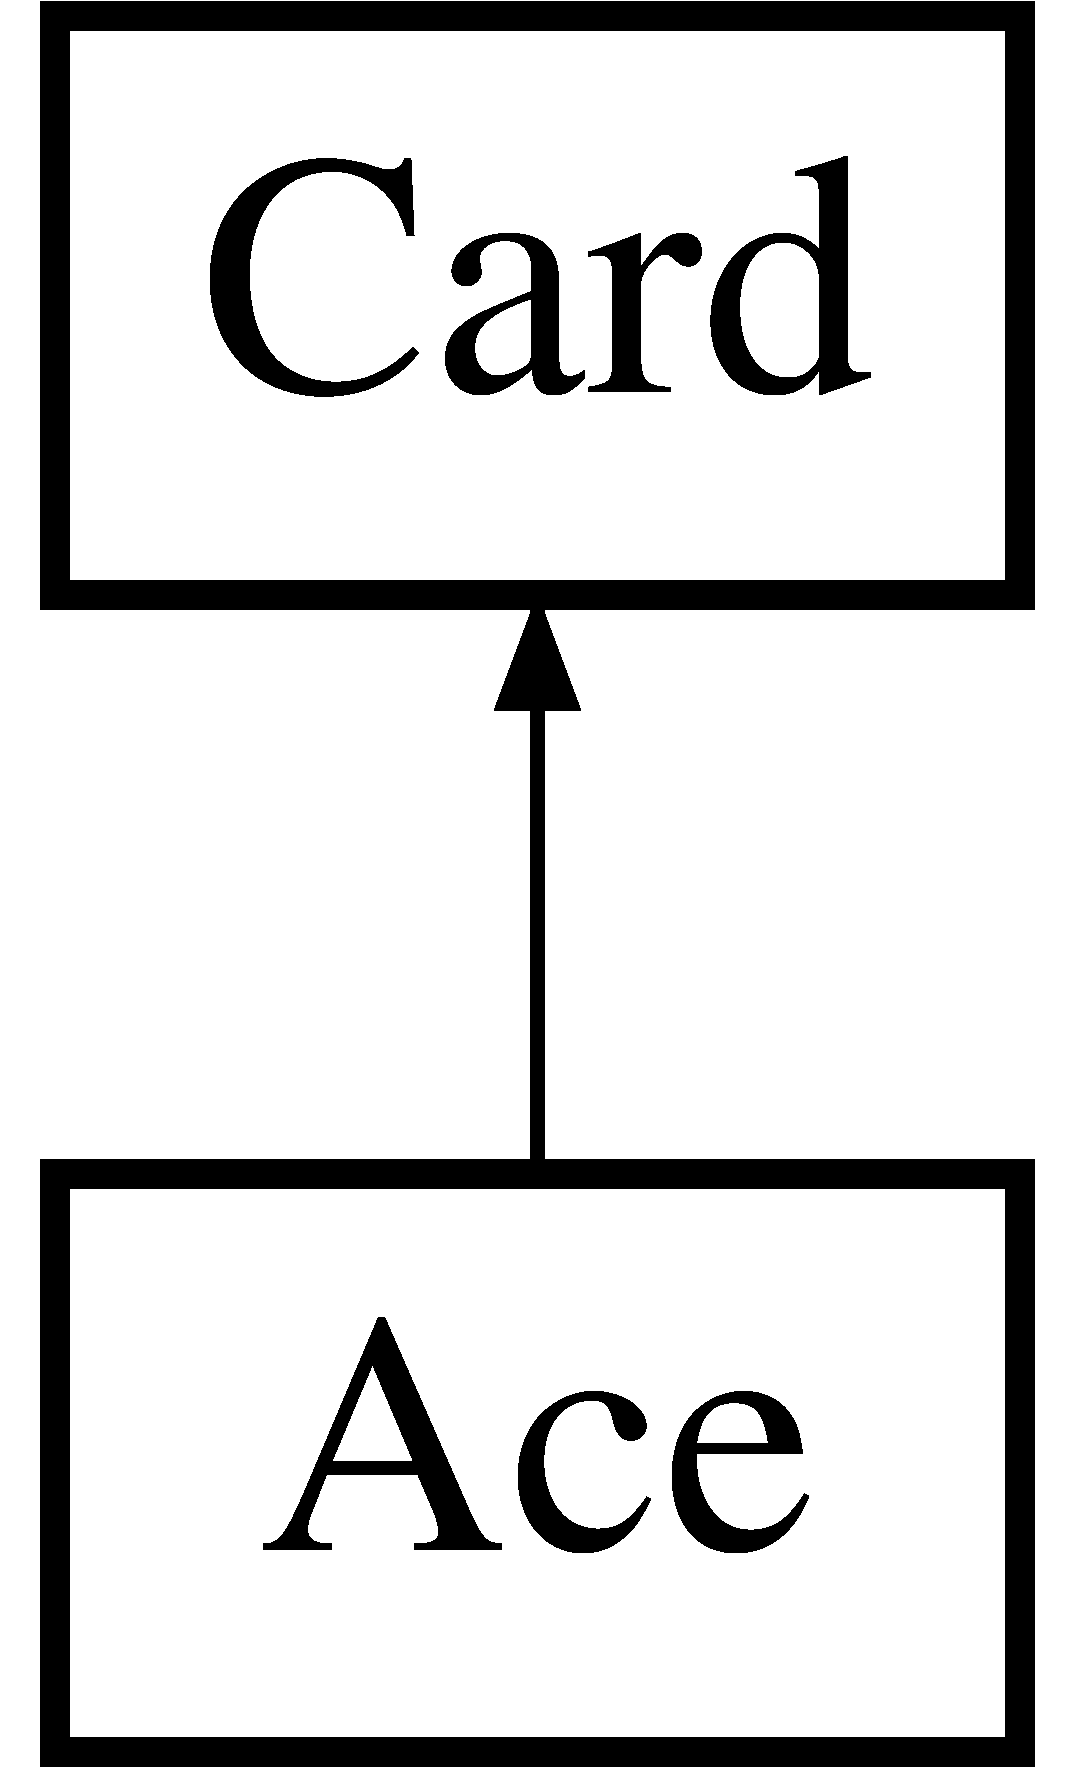
\includegraphics[height=2.000000cm]{class_ace}
\end{center}
\end{figure}
\subsection*{Public Member Functions}
\begin{DoxyCompactItemize}
\item 
{\bfseries Ace} (int, Suit)\hypertarget{class_ace_a56ff024bb9b079f04cec836ac3ba389c}{}\label{class_ace_a56ff024bb9b079f04cec836ac3ba389c}

\item 
void {\bfseries Print\+Card} ()\hypertarget{class_ace_a050c43881616cd6bd2cccaf18cffca45}{}\label{class_ace_a050c43881616cd6bd2cccaf18cffca45}

\item 
int {\bfseries Get\+Value} ()\hypertarget{class_ace_adfb0f5e0a407d142b194ca3fc0c821a3}{}\label{class_ace_adfb0f5e0a407d142b194ca3fc0c821a3}

\item 
void {\bfseries Dec\+Value} ()\hypertarget{class_ace_ababf90507705afe181768744c2cf7831}{}\label{class_ace_ababf90507705afe181768744c2cf7831}

\item 
void {\bfseries Inc\+Value} ()\hypertarget{class_ace_ac6e447fe80821643237c71f92e73adcd}{}\label{class_ace_ac6e447fe80821643237c71f92e73adcd}

\item 
bool {\bfseries Is\+Low} ()\hypertarget{class_ace_a8aa71eb43584d2e6cf56809d2b13b562}{}\label{class_ace_a8aa71eb43584d2e6cf56809d2b13b562}

\end{DoxyCompactItemize}
\subsection*{Public Attributes}
\begin{DoxyCompactItemize}
\item 
bool {\bfseries m\+\_\+b\+Low\+Val}\hypertarget{class_ace_a984604c0e554b5fd3e77e12082c25fd9}{}\label{class_ace_a984604c0e554b5fd3e77e12082c25fd9}

\end{DoxyCompactItemize}
\subsection*{Additional Inherited Members}


The documentation for this class was generated from the following file\+:\begin{DoxyCompactItemize}
\item 
Ace.\+h\end{DoxyCompactItemize}

\hypertarget{class_board}{}\section{Board Class Reference}
\label{class_board}\index{Board@{Board}}
\subsection*{Public Member Functions}
\begin{DoxyCompactItemize}
\item 
{\bfseries Board} (int, int, int)\hypertarget{class_board_a299f62d90ba5fbdc8440bfe308b8a8aa}{}\label{class_board_a299f62d90ba5fbdc8440bfe308b8a8aa}

\item 
\hyperlink{class_deck}{Deck} $\ast$ {\bfseries Make\+Game\+Deck} ()\hypertarget{class_board_a0716f4188a7a6d3d4cbeecbf19c2e1b8}{}\label{class_board_a0716f4188a7a6d3d4cbeecbf19c2e1b8}

\item 
void {\bfseries Game\+Menu} ()\hypertarget{class_board_a17cbef8bdb3bfedffd137834b53e1a83}{}\label{class_board_a17cbef8bdb3bfedffd137834b53e1a83}

\item 
void {\bfseries Offer\+Surrender} ()\hypertarget{class_board_ab6f39b1cec34664fe6d97697d31a898a}{}\label{class_board_ab6f39b1cec34664fe6d97697d31a898a}

\item 
void {\bfseries Award\+Insurance} ()\hypertarget{class_board_ad13e0d28f17bbd00bac5449a88ed7f2e}{}\label{class_board_ad13e0d28f17bbd00bac5449a88ed7f2e}

\item 
void {\bfseries Get\+Player\+Bets} ()\hypertarget{class_board_a375b51bf1380bdd7b204d8229f16e331}{}\label{class_board_a375b51bf1380bdd7b204d8229f16e331}

\item 
void {\bfseries Reward\+Players} ()\hypertarget{class_board_a4a512138d509b89f282f6eb17e02f24c}{}\label{class_board_a4a512138d509b89f282f6eb17e02f24c}

\item 
void {\bfseries Reset\+Player\+Bets} ()\hypertarget{class_board_a8ad211cf1d6e8bb62ae4488a6c6f50f3}{}\label{class_board_a8ad211cf1d6e8bb62ae4488a6c6f50f3}

\item 
void {\bfseries Deal\+Starting\+Hands} ()\hypertarget{class_board_a7a70fb73a8b8c638a3f93cf35f6a1e0a}{}\label{class_board_a7a70fb73a8b8c638a3f93cf35f6a1e0a}

\item 
\hyperlink{class_hand}{Hand} $\ast$ {\bfseries Make\+Starting\+Hand} ()\hypertarget{class_board_ad29b983eebabef3095da208b5d2c844a}{}\label{class_board_ad29b983eebabef3095da208b5d2c844a}

\item 
void {\bfseries Deal\+Card} (int, int)\hypertarget{class_board_ab9bf3b49f366c7b704d07688a6974078}{}\label{class_board_ab9bf3b49f366c7b704d07688a6974078}

\item 
void {\bfseries Split\+Hand} (\hyperlink{class_player}{Player} $\ast$, int)\hypertarget{class_board_af5fd0572e836460a3dbaca00928b89d7}{}\label{class_board_af5fd0572e836460a3dbaca00928b89d7}

\item 
void {\bfseries Print\+All\+Players} ()\hypertarget{class_board_aeb20716c3439b374c21bc7875e3fd92a}{}\label{class_board_aeb20716c3439b374c21bc7875e3fd92a}

\item 
void {\bfseries Print\+Dealer} (bool)\hypertarget{class_board_abb4069cf818d0f69e45a143b8200653d}{}\label{class_board_abb4069cf818d0f69e45a143b8200653d}

\item 
void {\bfseries Play\+Hands} (\hyperlink{class_player}{Player} $\ast$)\hypertarget{class_board_a97d21d0a6e7d0c298fb4188f3db01336}{}\label{class_board_a97d21d0a6e7d0c298fb4188f3db01336}

\item 
void {\bfseries Check\+Split} (\hyperlink{class_player}{Player} $\ast$)\hypertarget{class_board_a2c172c3d95827ebb463119ebf02beeaf}{}\label{class_board_a2c172c3d95827ebb463119ebf02beeaf}

\item 
void {\bfseries Clear\+Board} ()\hypertarget{class_board_aaab572b0a79a18e024aa70c9415a3c10}{}\label{class_board_aaab572b0a79a18e024aa70c9415a3c10}

\item 
bool {\bfseries Start\+Game} ()\hypertarget{class_board_adaecf6c1a1d833fd3038b91adf3ebc80}{}\label{class_board_adaecf6c1a1d833fd3038b91adf3ebc80}

\item 
void {\bfseries End\+Game} ()\hypertarget{class_board_a853016ae9afa3ffaaf7e881833f5ff2a}{}\label{class_board_a853016ae9afa3ffaaf7e881833f5ff2a}

\item 
void {\bfseries Start\+Round} ()\hypertarget{class_board_a1955daeb9befd1046a89135b8ec13a72}{}\label{class_board_a1955daeb9befd1046a89135b8ec13a72}

\item 
void {\bfseries Play\+Dealer} ()\hypertarget{class_board_ac15eb2363c6f318651511279b3470b55}{}\label{class_board_ac15eb2363c6f318651511279b3470b55}

\item 
void {\bfseries Print\+Winners} ()\hypertarget{class_board_a7c157ee7f34fc9d926b3dcf6e3f622ae}{}\label{class_board_a7c157ee7f34fc9d926b3dcf6e3f622ae}

\item 
void {\bfseries Check\+Deck} ()\hypertarget{class_board_ab4dd449a0bd9b44ba3cb05aee3d2671f}{}\label{class_board_ab4dd449a0bd9b44ba3cb05aee3d2671f}

\item 
void {\bfseries Offer\+Insurance} ()\hypertarget{class_board_a3300c8829b3f6edf37821b3b08491e71}{}\label{class_board_a3300c8829b3f6edf37821b3b08491e71}

\item 
bool {\bfseries Dealer\+Has\+BJ} ()\hypertarget{class_board_a76a78c90233a725e706feaf8d2ff542a}{}\label{class_board_a76a78c90233a725e706feaf8d2ff542a}

\end{DoxyCompactItemize}
\subsection*{Public Attributes}
\begin{DoxyCompactItemize}
\item 
\hyperlink{class_deck}{Deck} $\ast$ {\bfseries m\+\_\+game\+Deck}\hypertarget{class_board_ada80a0972dfb2b375ad2eb511fd279a8}{}\label{class_board_ada80a0972dfb2b375ad2eb511fd279a8}

\item 
int {\bfseries m\+\_\+n\+Players}\hypertarget{class_board_a97a72d923bd0e2700f4b14a7310f9654}{}\label{class_board_a97a72d923bd0e2700f4b14a7310f9654}

\item 
int {\bfseries m\+\_\+n\+Decks}\hypertarget{class_board_a5e1be4593464a9cce5686f1e270336b3}{}\label{class_board_a5e1be4593464a9cce5686f1e270336b3}

\item 
int {\bfseries m\+\_\+initial\+Pot}\hypertarget{class_board_a58d873cc5cd6f53b864d78dc24fa79b6}{}\label{class_board_a58d873cc5cd6f53b864d78dc24fa79b6}

\item 
std\+::map$<$ int, \hyperlink{class_player}{Player} $\ast$ $>$ {\bfseries m\+\_\+players}\hypertarget{class_board_a1f6a9b7c28344b393ec4e262a7869259}{}\label{class_board_a1f6a9b7c28344b393ec4e262a7869259}

\item 
int {\bfseries m\+\_\+option}\hypertarget{class_board_a49016c4ad23c494dcae6147aa9d6f975}{}\label{class_board_a49016c4ad23c494dcae6147aa9d6f975}

\item 
bool {\bfseries m\+\_\+b\+Play}\hypertarget{class_board_a01c952bc01bdf1f11ca4564ba74eb54d}{}\label{class_board_a01c952bc01bdf1f11ca4564ba74eb54d}

\item 
std\+::vector$<$ \hyperlink{class_player}{Player} $\ast$ $>$ {\bfseries m\+\_\+round\+Winners}\hypertarget{class_board_a7efb156cd4173c8d20511140f0428be7}{}\label{class_board_a7efb156cd4173c8d20511140f0428be7}

\item 
bool {\bfseries m\+\_\+b\+Push}\hypertarget{class_board_ae04975c508016ffd956a0b777f875625}{}\label{class_board_ae04975c508016ffd956a0b777f875625}

\item 
bool {\bfseries m\+\_\+b\+Dealer\+BJ}\hypertarget{class_board_a62f8285f2e20e1d69ea373af8a950892}{}\label{class_board_a62f8285f2e20e1d69ea373af8a950892}

\end{DoxyCompactItemize}


The documentation for this class was generated from the following files\+:\begin{DoxyCompactItemize}
\item 
Board.\+h\item 
Board.\+cpp\end{DoxyCompactItemize}

\hypertarget{class_card}{}\section{Card Class Reference}
\label{class_card}\index{Card@{Card}}
Inheritance diagram for Card\+:\begin{figure}[H]
\begin{center}
\leavevmode
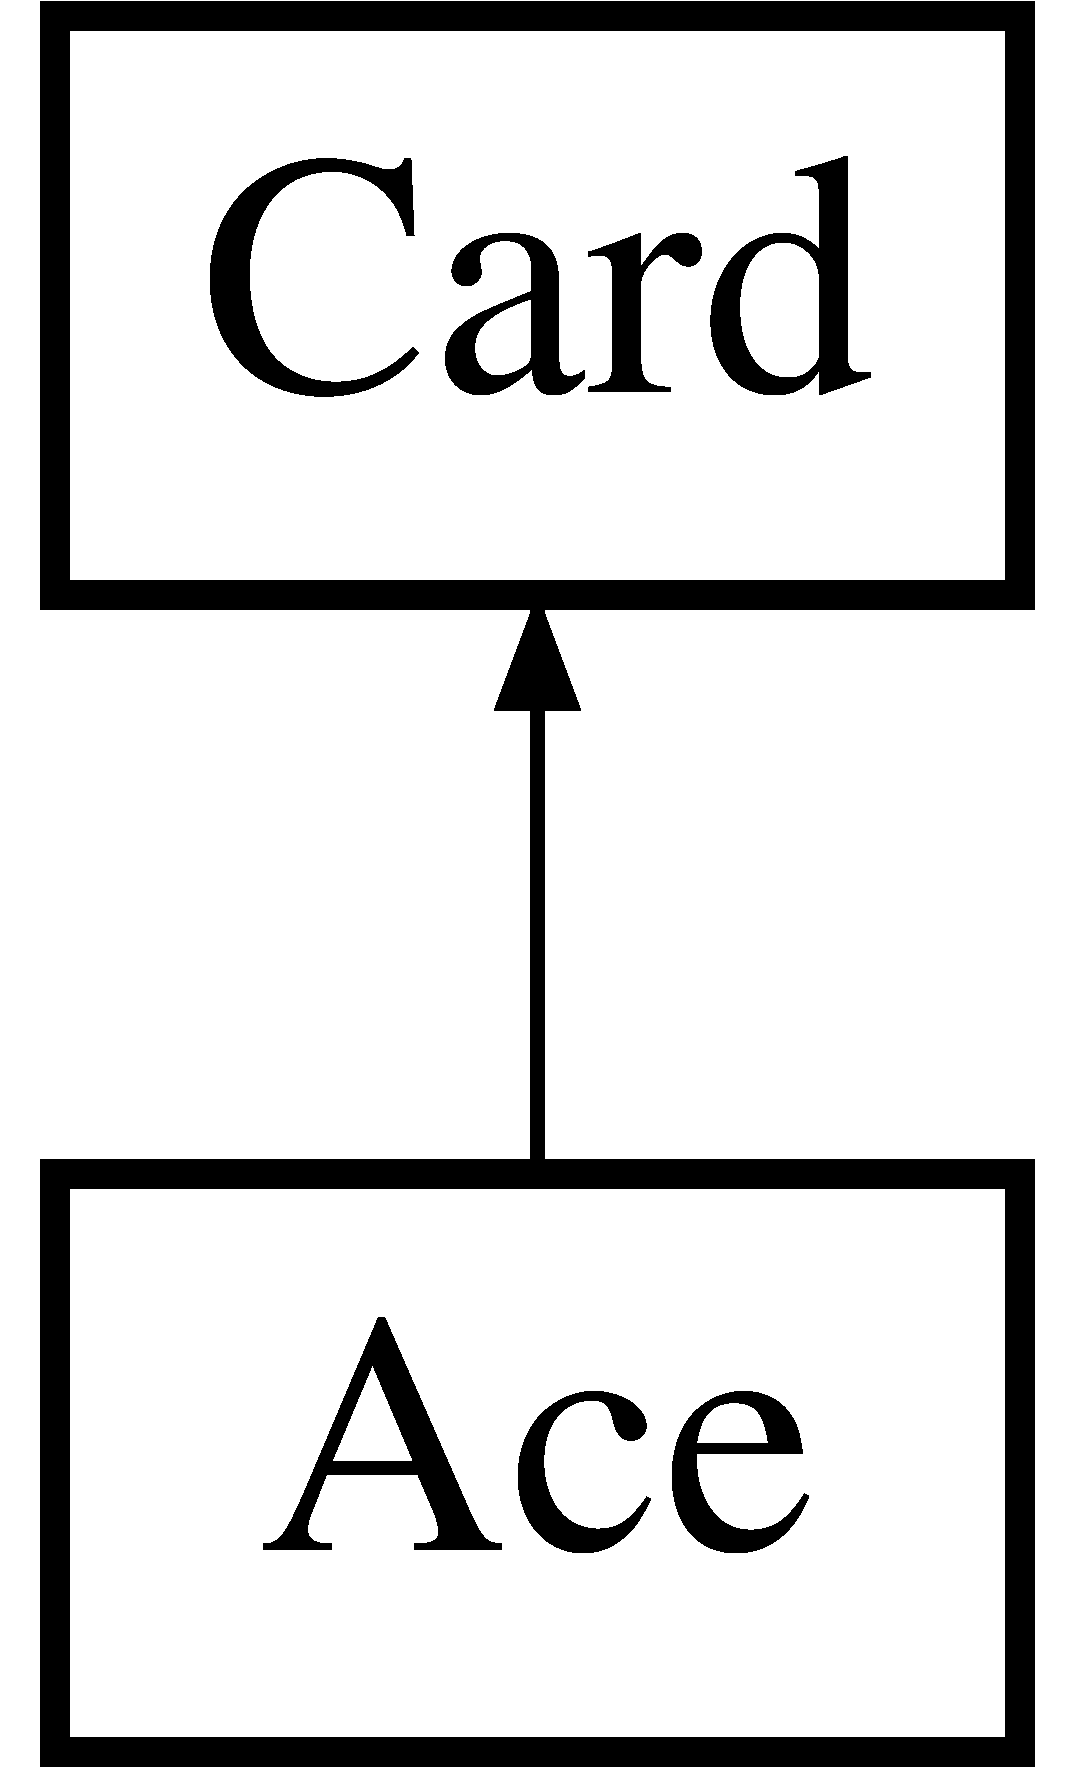
\includegraphics[height=2.000000cm]{class_card}
\end{center}
\end{figure}
\subsection*{Public Types}
\begin{DoxyCompactItemize}
\item 
enum {\bfseries Suit} \{ {\bfseries Club} = 0, 
{\bfseries Diamond} = 1, 
{\bfseries Spade} = 2, 
{\bfseries Heart} = 3
 \}\hypertarget{class_card_a5725a8e05afab8cd2f555bd81b069860}{}\label{class_card_a5725a8e05afab8cd2f555bd81b069860}

\end{DoxyCompactItemize}
\subsection*{Public Member Functions}
\begin{DoxyCompactItemize}
\item 
{\bfseries Card} (int, Suit)\hypertarget{class_card_aa403413f072507d2b985ab0a89d58ec5}{}\label{class_card_aa403413f072507d2b985ab0a89d58ec5}

\item 
virtual void {\bfseries Print\+Card} ()\hypertarget{class_card_af8d609d9fcbd761b9cf745bbbd3b709a}{}\label{class_card_af8d609d9fcbd761b9cf745bbbd3b709a}

\item 
virtual int {\bfseries Get\+Value} ()\hypertarget{class_card_ac1b08be5c93e652100bc993ce91c988d}{}\label{class_card_ac1b08be5c93e652100bc993ce91c988d}

\item 
virtual void {\bfseries Dec\+Value} ()\hypertarget{class_card_a72046d7f7bc4a33b69f9eb0bb154fa70}{}\label{class_card_a72046d7f7bc4a33b69f9eb0bb154fa70}

\item 
virtual bool {\bfseries Is\+Low} ()\hypertarget{class_card_ade427b5133fd8815fd0d5dcd0d097c84}{}\label{class_card_ade427b5133fd8815fd0d5dcd0d097c84}

\end{DoxyCompactItemize}
\subsection*{Public Attributes}
\begin{DoxyCompactItemize}
\item 
int {\bfseries m\+\_\+value}\hypertarget{class_card_a232ecb6ad51aa9684917af229a42988e}{}\label{class_card_a232ecb6ad51aa9684917af229a42988e}

\item 
Suit {\bfseries m\+\_\+suit}\hypertarget{class_card_a5eafb96c143a0010ce5ca155182a0b56}{}\label{class_card_a5eafb96c143a0010ce5ca155182a0b56}

\end{DoxyCompactItemize}


The documentation for this class was generated from the following files\+:\begin{DoxyCompactItemize}
\item 
Card.\+h\item 
Card.\+cpp\end{DoxyCompactItemize}

\hypertarget{class_deck}{}\section{Deck Class Reference}
\label{class_deck}\index{Deck@{Deck}}
\subsection*{Public Member Functions}
\begin{DoxyCompactItemize}
\item 
void {\bfseries Initialize\+Set} ()\hypertarget{class_deck_a0fea69180a61a2bb810ca18698ebc119}{}\label{class_deck_a0fea69180a61a2bb810ca18698ebc119}

\item 
void {\bfseries Shuffle} ()\hypertarget{class_deck_a1ed471063f40cb91c7e6786aa21737ef}{}\label{class_deck_a1ed471063f40cb91c7e6786aa21737ef}

\item 
\hyperlink{class_card}{Card} $\ast$ {\bfseries Deal\+Card} ()\hypertarget{class_deck_af4e4938969948cb4a471655cc4da3c90}{}\label{class_deck_af4e4938969948cb4a471655cc4da3c90}

\item 
{\bfseries Deck} (int)\hypertarget{class_deck_a5487610d44f13d27ef54c930e2bdadf9}{}\label{class_deck_a5487610d44f13d27ef54c930e2bdadf9}

\end{DoxyCompactItemize}
\subsection*{Public Attributes}
\begin{DoxyCompactItemize}
\item 
std\+::vector$<$ \hyperlink{class_card}{Card} $\ast$ $>$ {\bfseries m\+\_\+deck}\hypertarget{class_deck_ac27728877c50e97028566f9cb774408b}{}\label{class_deck_ac27728877c50e97028566f9cb774408b}

\item 
int {\bfseries m\+\_\+n\+Sets}\hypertarget{class_deck_af52c03d790a3182c7325d528839cd640}{}\label{class_deck_af52c03d790a3182c7325d528839cd640}

\end{DoxyCompactItemize}


The documentation for this class was generated from the following files\+:\begin{DoxyCompactItemize}
\item 
Deck.\+h\item 
Deck.\+cpp\end{DoxyCompactItemize}

\hypertarget{class_hand}{}\section{Hand Class Reference}
\label{class_hand}\index{Hand@{Hand}}
\subsection*{Public Member Functions}
\begin{DoxyCompactItemize}
\item 
{\bfseries Hand} (int)\hypertarget{class_hand_abaa16c2ffcc48ac2368d79cf810df6c7}{}\label{class_hand_abaa16c2ffcc48ac2368d79cf810df6c7}

\item 
int {\bfseries Sum\+Hand} ()\hypertarget{class_hand_adf9ecdee4a292e32dfee8a2da9c00589}{}\label{class_hand_adf9ecdee4a292e32dfee8a2da9c00589}

\item 
bool {\bfseries Print\+Hand} ()\hypertarget{class_hand_a1bb9cd4961231d7708fdeea731fe5a2e}{}\label{class_hand_a1bb9cd4961231d7708fdeea731fe5a2e}

\item 
void {\bfseries Dump\+Hand} ()\hypertarget{class_hand_aed8546ecef6466d591fe292b45692f74}{}\label{class_hand_aed8546ecef6466d591fe292b45692f74}

\item 
bool {\bfseries Dec\+Ace} ()\hypertarget{class_hand_a434f32de60bcdf7c795537b361658de5}{}\label{class_hand_a434f32de60bcdf7c795537b361658de5}

\item 
bool {\bfseries Can\+Split} ()\hypertarget{class_hand_a2933483fe779dddd638b8a5b6f809bb9}{}\label{class_hand_a2933483fe779dddd638b8a5b6f809bb9}

\end{DoxyCompactItemize}
\subsection*{Public Attributes}
\begin{DoxyCompactItemize}
\item 
std\+::vector$<$ \hyperlink{class_card}{Card} $\ast$ $>$ {\bfseries m\+\_\+hand}\hypertarget{class_hand_a13a8d342aac9dc2f7373ea7f5a6c62c1}{}\label{class_hand_a13a8d342aac9dc2f7373ea7f5a6c62c1}

\item 
int {\bfseries m\+\_\+hand\+ID}\hypertarget{class_hand_ae9f101083045b9ef0b9d75872e550031}{}\label{class_hand_ae9f101083045b9ef0b9d75872e550031}

\end{DoxyCompactItemize}


The documentation for this class was generated from the following file\+:\begin{DoxyCompactItemize}
\item 
Hand.\+h\end{DoxyCompactItemize}

\hypertarget{class_player}{}\section{Player Class Reference}
\label{class_player}\index{Player@{Player}}
\subsection*{Public Member Functions}
\begin{DoxyCompactItemize}
\item 
{\bfseries Player} (int, int)\hypertarget{class_player_a6f57cdacb88f4c3c800c1fbf591ed28d}{}\label{class_player_a6f57cdacb88f4c3c800c1fbf591ed28d}

\item 
void {\bfseries Surrender} ()\hypertarget{class_player_af8c9588488fcfdbd0735506300576722}{}\label{class_player_af8c9588488fcfdbd0735506300576722}

\item 
void {\bfseries Split} (int index)\hypertarget{class_player_a3a627672714563333c44d83faf8a2696}{}\label{class_player_a3a627672714563333c44d83faf8a2696}

\item 
void {\bfseries Add\+Hand} (\hyperlink{class_hand}{Hand} $\ast$hand)\hypertarget{class_player_add15dd07cc4772d4509a49e31b04556b}{}\label{class_player_add15dd07cc4772d4509a49e31b04556b}

\item 
bool {\bfseries Print\+Hand} (int)\hypertarget{class_player_a2142881dd58bd5ac7a7ec75b958069e1}{}\label{class_player_a2142881dd58bd5ac7a7ec75b958069e1}

\item 
void {\bfseries Print\+Hands} ()\hypertarget{class_player_a31326f0143919f9d2412bf094f571a95}{}\label{class_player_a31326f0143919f9d2412bf094f571a95}

\item 
void {\bfseries Dump\+Hands} ()\hypertarget{class_player_a2b8128800c27146c8ecebbbf2d1f4ffa}{}\label{class_player_a2b8128800c27146c8ecebbbf2d1f4ffa}

\item 
bool {\bfseries Can\+Split} (int)\hypertarget{class_player_a228554349109ae4e44ee40209796bb16}{}\label{class_player_a228554349109ae4e44ee40209796bb16}

\item 
bool {\bfseries Has\+Black\+Jack} ()\hypertarget{class_player_ae7d44ce9ba3598f2e42ff3b8dbfa78a2}{}\label{class_player_ae7d44ce9ba3598f2e42ff3b8dbfa78a2}

\item 
void {\bfseries Award\+Insurance} ()\hypertarget{class_player_ab179fcfd238511fd52dd98a911483b7d}{}\label{class_player_ab179fcfd238511fd52dd98a911483b7d}

\item 
void {\bfseries Print\+Pot} ()\hypertarget{class_player_a1129e1688f9243b849a4707809d44d10}{}\label{class_player_a1129e1688f9243b849a4707809d44d10}

\item 
bool {\bfseries Place\+Bet} (int)\hypertarget{class_player_ac40c56a426208d1fd1a93d75830e8a88}{}\label{class_player_ac40c56a426208d1fd1a93d75830e8a88}

\item 
void {\bfseries Double\+Down} ()\hypertarget{class_player_aa9e61858c03da97d7f840935c69f2515}{}\label{class_player_aa9e61858c03da97d7f840935c69f2515}

\item 
void {\bfseries Buy\+Insurance} ()\hypertarget{class_player_ae1551ff1ab9b7421d9e1a2887c3bfc70}{}\label{class_player_ae1551ff1ab9b7421d9e1a2887c3bfc70}

\item 
void {\bfseries Add\+Winnings} (bool)\hypertarget{class_player_add0b1bdc9b4b8d0be111dc2ed42b23f3}{}\label{class_player_add0b1bdc9b4b8d0be111dc2ed42b23f3}

\item 
void {\bfseries Push\+Winnings} ()\hypertarget{class_player_a0b6e7be395b4974db2fe3875522d3966}{}\label{class_player_a0b6e7be395b4974db2fe3875522d3966}

\item 
void {\bfseries Reset\+Bets} ()\hypertarget{class_player_a250f1aa39f0bd26dd499a5708d400b56}{}\label{class_player_a250f1aa39f0bd26dd499a5708d400b56}

\item 
bool {\bfseries Can\+Double\+Down} ()\hypertarget{class_player_a38e44a9263556227594f509b3bbb6ed1}{}\label{class_player_a38e44a9263556227594f509b3bbb6ed1}

\item 
bool {\bfseries Can\+Buy\+Insur} ()\hypertarget{class_player_a5b2a2c6d52ef4d68043b649b94c1e260}{}\label{class_player_a5b2a2c6d52ef4d68043b649b94c1e260}

\item 
int {\bfseries Ace\+Pos} (int)\hypertarget{class_player_abfd18db1c47281948161454cf06eabc1}{}\label{class_player_abfd18db1c47281948161454cf06eabc1}

\item 
int {\bfseries Blackjack\+Pos} ()\hypertarget{class_player_a97c9f070e70e47691b0bdda9993040f2}{}\label{class_player_a97c9f070e70e47691b0bdda9993040f2}

\end{DoxyCompactItemize}
\subsection*{Public Attributes}
\begin{DoxyCompactItemize}
\item 
std\+::vector$<$ \hyperlink{class_hand}{Hand} $\ast$ $>$ {\bfseries m\+\_\+hand\+List}\hypertarget{class_player_ac4ef2a880d80f353a4a96391516d5629}{}\label{class_player_ac4ef2a880d80f353a4a96391516d5629}

\item 
int {\bfseries m\+\_\+player\+ID}\hypertarget{class_player_a82caa9879f5233e641dda10a41d9186f}{}\label{class_player_a82caa9879f5233e641dda10a41d9186f}

\item 
\hyperlink{class_pot}{Pot} $\ast$ {\bfseries m\+\_\+pot}\hypertarget{class_player_a16264ed3055966735e372567d594d538}{}\label{class_player_a16264ed3055966735e372567d594d538}

\item 
bool {\bfseries m\+\_\+b\+Surrender}\hypertarget{class_player_ae7736ed56c6057fbaf60330a110dd818}{}\label{class_player_ae7736ed56c6057fbaf60330a110dd818}

\end{DoxyCompactItemize}


The documentation for this class was generated from the following files\+:\begin{DoxyCompactItemize}
\item 
Player.\+h\item 
Player.\+cpp\end{DoxyCompactItemize}

\hypertarget{class_pot}{}\section{Pot Class Reference}
\label{class_pot}\index{Pot@{Pot}}
\subsection*{Public Member Functions}
\begin{DoxyCompactItemize}
\item 
{\bfseries Pot} (int)\hypertarget{class_pot_ae1fecaba6730af51a13cf57726f2e304}{}\label{class_pot_ae1fecaba6730af51a13cf57726f2e304}

\item 
bool {\bfseries Place\+Bet} (int)\hypertarget{class_pot_a9932b87968829937f62d7dd60e11046e}{}\label{class_pot_a9932b87968829937f62d7dd60e11046e}

\item 
void {\bfseries Double\+Down} ()\hypertarget{class_pot_afccb26a065de8c5192acd72b1dff217d}{}\label{class_pot_afccb26a065de8c5192acd72b1dff217d}

\item 
void {\bfseries Buy\+Insurance} (int)\hypertarget{class_pot_a5e1e06ffa0cd7a74087297a84cfeb17f}{}\label{class_pot_a5e1e06ffa0cd7a74087297a84cfeb17f}

\item 
void {\bfseries Add\+Winnings} (bool)\hypertarget{class_pot_afa6a1574446fdc8fb3450095e6586944}{}\label{class_pot_afa6a1574446fdc8fb3450095e6586944}

\item 
void {\bfseries Push\+Winnings} ()\hypertarget{class_pot_a9e3e905d1cf6759db2105dabf22fc454}{}\label{class_pot_a9e3e905d1cf6759db2105dabf22fc454}

\item 
bool {\bfseries Reset\+Bets} ()\hypertarget{class_pot_a7ec1ff4578b4cec267e652876297897f}{}\label{class_pot_a7ec1ff4578b4cec267e652876297897f}

\item 
bool {\bfseries Can\+Double\+Down} ()\hypertarget{class_pot_af6a1e26563014a493c1fd6b0c7d1f48e}{}\label{class_pot_af6a1e26563014a493c1fd6b0c7d1f48e}

\item 
bool {\bfseries Can\+Buy\+Insur} ()\hypertarget{class_pot_a7e13e6cdb743259fdb3784ec1272ab98}{}\label{class_pot_a7e13e6cdb743259fdb3784ec1272ab98}

\item 
void {\bfseries Print\+Pot} ()\hypertarget{class_pot_a1c3fde3bd8e004664efb06846ead92fc}{}\label{class_pot_a1c3fde3bd8e004664efb06846ead92fc}

\item 
void {\bfseries Print\+Bet} ()\hypertarget{class_pot_a770efd0511771dea454510cb89be354b}{}\label{class_pot_a770efd0511771dea454510cb89be354b}

\end{DoxyCompactItemize}
\subsection*{Public Attributes}
\begin{DoxyCompactItemize}
\item 
int {\bfseries m\+\_\+initial\+Pot}\hypertarget{class_pot_ac83f0f8076ae4581017b04acedb15162}{}\label{class_pot_ac83f0f8076ae4581017b04acedb15162}

\item 
int {\bfseries m\+\_\+cur\+Bet}\hypertarget{class_pot_a9387b52aafa588830e58056efb1df365}{}\label{class_pot_a9387b52aafa588830e58056efb1df365}

\item 
int {\bfseries m\+\_\+cur\+Pot}\hypertarget{class_pot_a3c53359bce49d08ad42378a40223ec76}{}\label{class_pot_a3c53359bce49d08ad42378a40223ec76}

\item 
int {\bfseries m\+\_\+cur\+Insurance}\hypertarget{class_pot_adc1c1fcd3be66dadeab0633fdbde460c}{}\label{class_pot_adc1c1fcd3be66dadeab0633fdbde460c}

\end{DoxyCompactItemize}


The documentation for this class was generated from the following files\+:\begin{DoxyCompactItemize}
\item 
Pot.\+h\item 
Pot.\+cpp\end{DoxyCompactItemize}

%--- End generated contents ---

% Index
\backmatter
\newpage
\phantomsection
\clearemptydoublepage
\addcontentsline{toc}{chapter}{Index}
\printindex

\end{document}
